\documentclass{article}

% preambulo:
\usepackage[utf8]{inputenc}
% caracteres utf8 (tildes, enie) sin tener que usar comandos

\usepackage[spanish, es-tabla, es-nodecimaldot]{babel} 
% texto automatico en espaniol
% "tabla" en vez de "cuadro"
% no reemplaza puntos decimales por comas

%% NO AGREGAR PAQUETES ANTES DE ESTO, ES IMPORTANTE QUE BABEL ESTE PRIMERO

%%%%%%%%%%%%%%%%%%%%%%%%%%%%%%%%%
%% PAQUETES EXTRA %%%%%%%%%%%%%%%
%%%%%%%%%%%%%%%%%%%%%%%%%%%%%%%%%

\usepackage{subfiles}

\usepackage{amsmath} % PAQUETES DE MATEMATICA
\usepackage{amsfonts}
\usepackage{amssymb}


\usepackage{steinmetz} % comando \phase{}
\usepackage{units} % permite usar nicefrac
\usepackage{graphicx} % importar imagenes
\usepackage{float} % posicion H para floats
\usepackage[colorinlistoftodos]{todonotes}


\usepackage[a4paper, total={6in, 8in}]{geometry} 
% margenes correctos en subarchivos

\setlength{\parindent}{10pt}			%cuanta sangria al principio de un parrafo
\usepackage{indentfirst}				%pone sangria al primer parrafo de una seccion

\usepackage{listings}

%%%%%%%%%%%%%%%%%%%%%%%%%%%%%%%%%%%%%%%%%%%%%%%%%%%%%%%%%%%
%% NO AGREGAR PAQUETES DESPUES DE ESTO, ES IMPORTANTE QUE HYPERREF ESTE ULTIMO
\usepackage[hidelinks]{hyperref} % hipervinculos sin cajitas rojas




\begin{document}

\newgeometry{} % margenes default para la caratula
% caratula:
\begin{titlepage}
\newcommand{\HRule}{\rule{\linewidth}{0.5mm}}
\center
\mbox{\textsc{\LARGE \bfseries {Instituto Tecnol\'ogico de Buenos Aires}}}\\[1.5cm]
\textsc{\Large 22.99 Laboratorio de Microprocesadores}\\[0.5cm]


\HRule \\[0.6cm]
{ \Huge \bfseries Guía de Ejercicios N$^{\circ}$2: Introducción a Kinetis}\\[0.4cm] % Title of your document
\HRule \\[1.5cm]


{\large

\emph{Grupo 2}\\
\vspace{3px}

\begin{tabular}{lr} 	
\textsc{M\'aspero}, Martina  & 57120 \\
\textsc{Mestanza}, Joaqu\'in Mat\'ias  & 58288 \\
\textsc{Nowik}, Ariel Santiago  & 58309 \\
\textsc{Regueira}, Marcelo Daniel  & 58300 \\
\end{tabular}

\vspace{20px}

\emph{Profesores}\\
\vspace{3px}
\textsc{Jacoby}, Daniel Andr\'es\\ 	
\textsc{Magliola}, Nicol\'as\\ 	

\vspace{100px}

\begin{tabular}{ll}

Presentado: & 22/08/2019\\

\end{tabular}

}

\vfill

\end{titlepage}

% cambio los margenes para el resto del documento
\newgeometry{left=2.5cm, top=2.5cm, right=2cm, bottom=2cm}

% indice:
\tableofcontents
\newpage

\section*{Ejercicio 1 - Documentación}
\addcontentsline{toc}{section}{Ejercicio 1 - Documentación}

\begin{itemize}
\item ¿En cuál número de pin del MCU se encuentra el puerto PTA12?
\end{itemize}
En el datasheet del MCU, la sección 5.3 ``K64 Pinouts'' figura 37, se indica que el puerto PTA12 es el pin 64.

\begin{itemize}
\item ¿Cuáles pines pueden funcionar como entradas analógicas?
\end{itemize}
En el datasheet del MCU, la sección 5.2 ``Unused analog interfaces'' tabla 57, indica el nombre del módulo y los pines asociados:

\begin{figure}[ht]
	\centering
	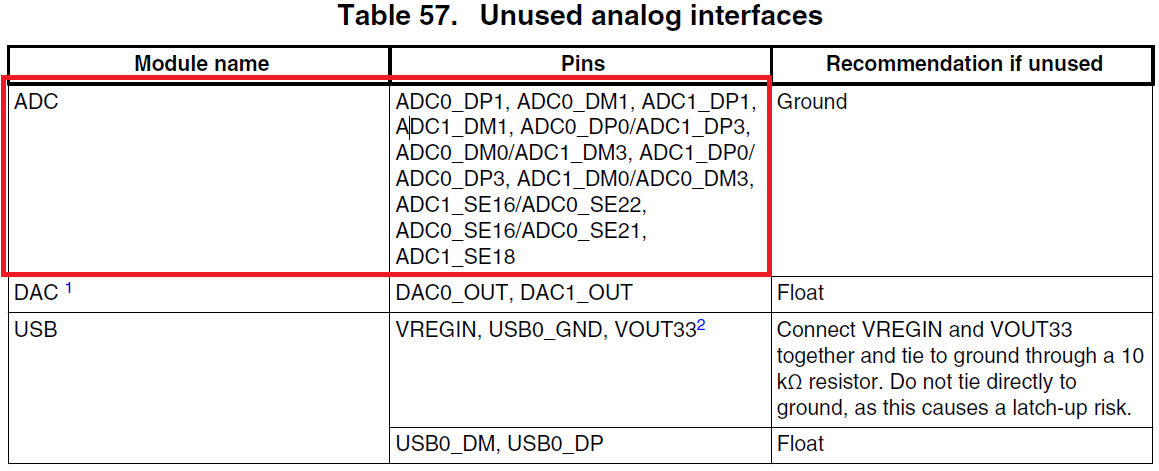
\includegraphics[width=0.8 \textwidth]
	{../Imagenes/TablaADC.png}
	\caption{Pines de entrada analógica}
	\label{fig:ej1}
\end{figure}

\begin{itemize}
\item ¿Cuántos pines del puerto PTE se encuentran efectivamente disponibles en este modelo de MCU?
\end{itemize}
En la guía de usuario del kit Freedom, sección 16 ``Input/output connectors'' se muestran los pintes accesibles en la placa de evaluación. Los pines disponibles de uso externo del puerto PTE son el PTE24, PTE25 y el PTE26.

\begin{itemize}
\item ¿Cuál es el rango de valores de tensión para detectar un 0 y un 1 lógico en un pin I/O? ¿Se puede enviar 5V a un pin?
\end{itemize}
En el datasheet del MCU, la sección 2.2.1 ``Voltage and current operating requirements'' tabla 1 se indican los márgenes de ruido correspondientes:

\begin{figure}[ht]
	\centering
	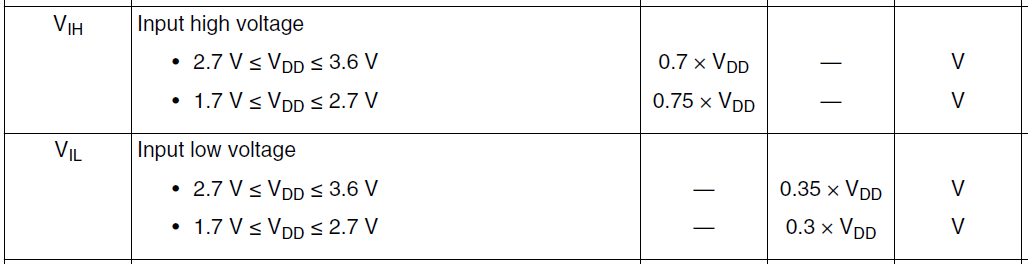
\includegraphics[width=0.8 \textwidth]
	{../Imagenes/TablaMargenes.png}
	\caption{Márgenes de ruido}
	\label{fig:ej1}
\end{figure}

Por otro lado, en el datasheet del MCU, la sección 1.4 ``Voltage and current operating ratings'', en el cuadro se indica que la máxima tensión de entrada a un pin I/O es de 5.5V.

\begin{itemize}
\item ¿Cuál es la máxima corriente que entrega un pin I/O?
\end{itemize}
En el datasheet del MCU, la sección 1.4 ``Voltage and current operating ratings'', en el cuadro se indica que la máxima corriente por un pin I/O es de 25mA.

\newpage

\section*{Ejercicio 2 - toolchain Kinetis}
\addcontentsline{toc}{section}{Ejercicio 2 - toolchain Kinetis}

Con el nivel de optimización original (None - O0), el código funciona normalmente. Con la opción Disassembly se puede obtener el fragmento de código de la función App\_run:

\begin{lstlisting}
          App_Run:
00000410:   push    {r7, lr}
00000412:   add     r7, sp, #0
00000414:   ldr     r0, [pc, #12]   ; (0x424 <App_Run+20>)
00000416:   bl      0x6b0 <delayLoop>
0000041a:   movs    r0, #154        ; 0x9a
0000041c:   bl      0x658 <gpioToggle>
00000420:   nop     
00000422:   pop     {r7, pc}
00000424:   rev     r0, r0
00000426:   lsls    r3, r3, #3
\end{lstlisting}

En el cual se observa que el compilador procesa la función delayloop correctamente. En cambio, utilizando la opción Optimize Most - O3, el compilador elimina esa función dado que bloquea el programa (y puede realizarse lo mismo con un timer). En consecuencia queda solamente el toogle corriendo todo el tiempo sin delay, por lo que no se llega a ver el blink.

\begin{lstlisting}
          App_Run:
00000418:   movs    r0, #154        ; 0x9a
0000041a:   b.w     0x614 <gpioToggle>
0000041e:   nop     
\end{lstlisting}

\newpage

\section*{Ejercicio 3 - Blink editado}
\addcontentsline{toc}{section}{Ejercicio 3 - Blink editado}

Para utilizar el LED verde del RGB, se modificó el define correspondiente a dicho puerto, en board.h:

\begin{lstlisting}
#define PIN_LED_GREEN   PORTNUM2PIN(PE,26) // PTE26
\end{lstlisting}

En base a esto, se modificó también el código en App.c:

\begin{lstlisting}
/* Funcion que se llama 1 vez, al comienzo del programa */
void App_Init (void)
{
    gpioMode(PIN_LED_GREEN, OUTPUT);
}

/* Funcion que se llama constantemente en un ciclo infinito */
void App_Run (void)
{
    delayLoop(4*3600000UL);
    gpioToggle(PIN_LED_GREEN);
}
\end{lstlisting}

El valor en delayloop se modificó por regla de 3, dado que es un while que incrementa una variable, y para conocer el tiempo que demora se midió el del código de blink con el osciloscopio, que era delayloop(4000000UL). La forma más adecuada de implementar un retardo en el cambio de estado de un pin sería utilizando un timer.

\newpage

\section*{Ejercicio 4 - Pul2Switch}
\addcontentsline{toc}{section}{Ejercicio 4 - Pul2Switch}

Se le agregó un delay a la función para esperar el tiempo que tarda uno en retirar el dedo del botón y evitar efecto rebote, para que el LED solo cambie de estado una vez al presionar. Consideramos que lo ideal es usar una interrupción para detectar cuando se presiona el pulsador que estar revisando todo el tiempo.
En board.h se agregó:

\begin{lstlisting}
#define PIN_LED_GREEN   PORTNUM2PIN(PE,26) // PTE26
#define PIN_SW3         PORTNUM2PIN(PA,4) // PTA4
\end{lstlisting}

En App.c se modificaron las funciones App\_Init y App\_Run:

\begin{lstlisting}
/* Funcion que se llama 1 vez, al comienzo del programa */
void App_Init (void)
{
    gpioMode(PIN_LED_GREEN, OUTPUT); // Configuro LED GREEN como salida
    gpioMode(PIN_SW3, INPUT);        // COnfiguro SW3 como entrada
}

/* Funcion que se llama constantemente en un ciclo infinito */
void App_Run (void)
{
	static int estado = HIGH;
	int estado_viejo = estado;
	estado = gpioRead(PIN_SW3);
	if((estado_viejo == HIGH)&&(estado == LOW)){
		delayLoop(360000UL); // Delay antirebote basico
		gpioToggle(PIN_LED_GREEN);
	}
}
\end{lstlisting}

En el caso donde se utiliza SW2, en el esquemático de la placa la resistencia de pull-up figura como DNP (do not populate). Es decir, que no viene montada en el PCB, por lo que si en el programa no se configura como INPUT\_PULLUP no va a funcionar.

\begin{figure}[ht]
	\centering
	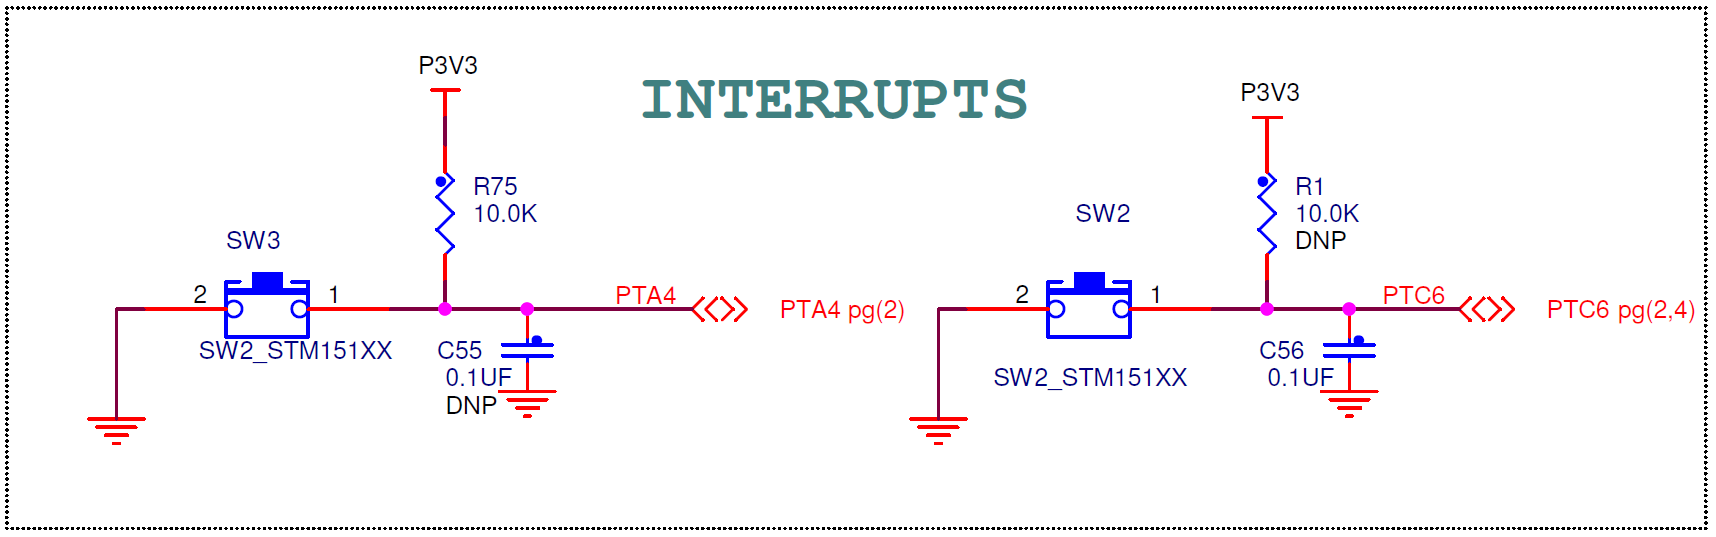
\includegraphics[width=0.7 \textwidth]
	{../Imagenes/SW2_DNP.png}
	\caption{Esquemático del SW2 interno}
	\label{fig:ej1}
\end{figure}

El código modificado para estos fines se muestra a continuación.

En board.h:

\begin{lstlisting}
#define PIN_LED_GREEN   PORTNUM2PIN(PE,26) // PTE26
#define PIN_SW2         PORTNUM2PIN(PC,6) // PTC6
\end{lstlisting}

En App.c se modificaron las funciones App\_Init y App\_Run:

\begin{lstlisting}
/* Funcion que se llama 1 vez, al comienzo del programa */
void App_Init (void)
{
    gpioMode(PIN_LED_GREEN, OUTPUT); // Configuro LED GREEN como salida
    gpioMode(PIN_SW2, INPUT_PULLUP); // COnfiguro SW2 como entrada con pull-up interno
}

/* Funcion que se llama constantemente en un ciclo infinito */
void App_Run (void)
{
	static int estado = HIGH;
	int estado_viejo = estado;
	estado = gpioRead(PIN_SW2);
	if((estado_viejo == HIGH)&&(estado == LOW)){
		delayLoop(360000UL); // Delay antirebote basico
		gpioToggle(PIN_LED_GREEN);
	}
}
\end{lstlisting}

\newpage

\section*{Ejercicio 5 - Interfaz externa}
\addcontentsline{toc}{section}{Ejercicio 5 - Interfaz externa}

Se conectaron en un protoboard un pulsador al pin PTC9 y un LED amarillo al pin PTB23. El código modificado se muestra a continuación.

En board.h:

\begin{lstlisting}
// Extern LED
#define LED_YELLOW	PORTNUM2PIN(PB,23) // PTB23

// Extern SW
#define SW_EXT	PORTNUM2PIN(PC,9) // PTC9
\end{lstlisting}

Se modificó además en App.c:

\begin{lstlisting}
/* Funcion que se llama 1 vez, al comienzo del programa */
void App_Init (void)
{
    gpioMode(LED_YELLOW, OUTPUT);
    gpioMode(SW_EXT, INPUT_PULLUP);
    gpioWrite(LED_YELLOW, HIGH); // Para ver que ande
}

/* Funcion que se llama constantemente en un ciclo infinito */
void App_Run (void)
{
	static int estado = HIGH;
	int estado_viejo = estado;
	estado = gpioRead(SW_EXT);
	if((estado_viejo == HIGH)&&(estado == LOW)){
		delayLoop(800000UL);
		gpioToggle(LED_YELLOW);
	}
}
\end{lstlisting}

La segunda conexión sugerida no se puede efectuar en la placa de evaluación, dado que el pin PTA0 es utilizado por una señal del debugger de la placa.

\begin{figure}[ht]
	\centering
	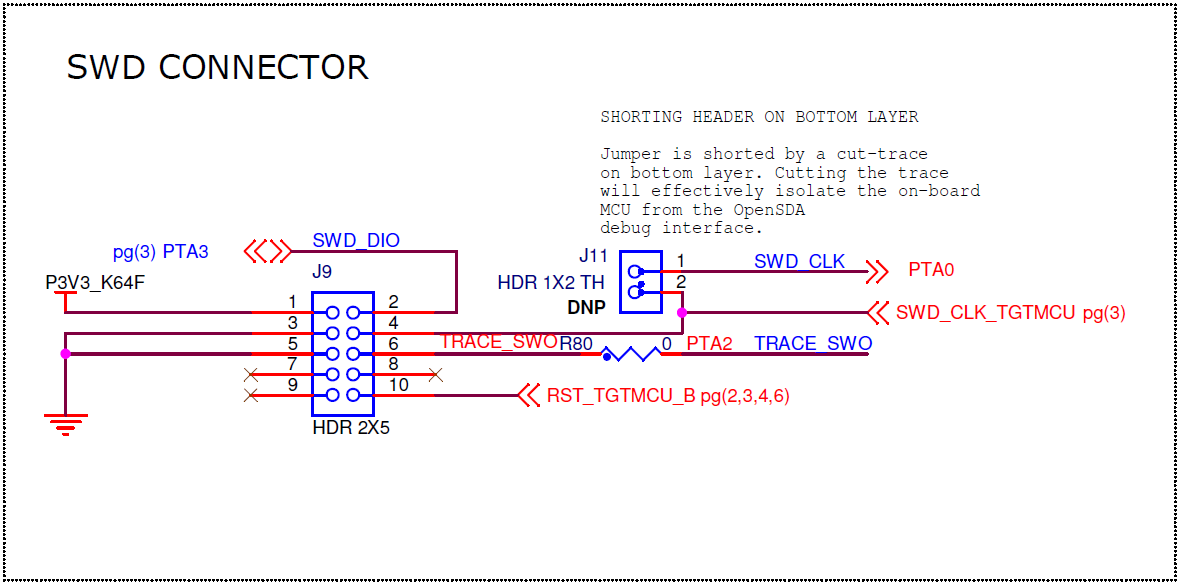
\includegraphics[width=0.8 \textwidth]
	{../Imagenes/PTA0.png}
	\caption{Conexionado interno del PTA0}
	\label{fig:ej1}
\end{figure}

\newpage

\section*{Ejercicio 6 - Baliza}
\addcontentsline{toc}{section}{Ejercicio 6 - Baliza}

Para leer el estado del SW3 periódicamente sin utilizar interrupciones, se colocó un delay de 10ms. Si se presionó, se habilita la baliza, y como el delay es de 10ms, en cada centena de la variable timer (que se incrementa por ciclo de 10ms en forma unitaria) se cambia el estado del LED de la baliza. Nuevamente, el valor de delayloop se calculó mediante regla de 3.
Modificando los defines en board.h:

\begin{lstlisting}
// On Board User LEDs
#define PIN_LED_RED     PORTNUM2PIN(PB,22) // PTB22

// On Board User Switches
#define PIN_SW3         PORTNUM2PIN(PA,4) // PTA4

// Extern LED
#define LED_YELLOW	PORTNUM2PIN(PB,23) // PTB23
\end{lstlisting}

Finalmente, en App.c:

\begin{lstlisting}

/* Funcion que se llama 1 vez, al comienzo del programa */
void App_Init (void)
{
	gpioMode(PIN_SW3, INPUT);
    gpioMode(LED_YELLOW, OUTPUT);
    gpioMode(PIN_LED_RED, OUTPUT);
    gpioWrite(LED_YELLOW, LOW);
    gpioWrite(PIN_LED_RED, HIGH);
}

/* Funcion que se llama constantemente en un ciclo infinito */
void App_Run (void)
{
	static int timer = 0;
	static int estado = HIGH;
	static int baliza = LOW; // Inicialmente apagado
	int estado_viejo = estado;
	timer++; // Cada 10ms
	estado = gpioRead(PIN_SW3);
	if((estado_viejo == HIGH)&&(estado == LOW)){
		if(baliza == LOW){
			baliza = HIGH;
		}else{
			baliza = LOW;
		}
	}

	delayLoop(143000UL); // 10ms de pausa

	switch(baliza){
	case LOW:
		if(gpioRead(PIN_LED_RED) == LOW){
		    gpioWrite(LED_YELLOW, LOW);
		    gpioWrite(PIN_LED_RED, HIGH);
		}
		break;
	case HIGH:
		if(timer % 100 == 0){ // Cada 1 segundo debido al delayloop
			gpioToggle(LED_YELLOW);
		}
		if(gpioRead(PIN_LED_RED) == HIGH){
			gpioWrite(PIN_LED_RED, LOW);
		}
		break;
	default:
		// Nada
		break;
	}
}
\end{lstlisting}

\end{document}
